\documentclass[UTF8]{ctexart}
\usepackage{geometry, CJKutf8}
\geometry{margin=1.5cm, vmargin={0pt,1cm}}
\setlength{\topmargin}{-1cm}
\setlength{\paperheight}{29.7cm}
\setlength{\textheight}{25.3cm}

% useful packages.
\usepackage{amsfonts}
\usepackage{graphicx}
\usepackage{amsmath}
\usepackage{amssymb}
\usepackage{amsthm}
\usepackage{enumerate}
\usepackage{graphicx}
\usepackage{multicol}
\usepackage{fancyhdr}
\usepackage{layout}
\usepackage{listings}
\usepackage{xcolor}
\usepackage{float, caption}
\usepackage{titling}

\pretitle{\begin{center}\Huge\bfseries}
\posttitle{\end{center}}
\preauthor{\begin{center}\Large\scshape}
\postauthor{\end{center}}
\predate{\begin{center}\large}
\postdate{\end{center}}

\lstset{
    language=C++, % 设置语言
    basicstyle=\ttfamily\small, % 基本样式
    keywordstyle=\color{blue}, % 关键字颜色
    commentstyle=\color{cyan}, % 注释颜色
    stringstyle=\color{red}, % 字符串颜色
    numberstyle=\tiny\color{gray}, % 行号样式
    numbers=left, % 行号位置
    stepnumber=1, % 行号步长
    numbersep=5pt, % 行号与代码间距
    backgroundcolor=\color{white}, % 代码背景色
    showspaces=false, % 显示空格
    showstringspaces=false, % 显示字符串中的空格
    showtabs=false, % 显示制表符
    frame=single, % 代码框
    tabsize=4, % 制表符宽度
    captionpos=b, % 标题位置
    breaklines=true, % 自动换行
    breakatwhitespace=false, % 仅在空格处换行
    escapeinside={\%*}{*)} ,% 特殊字符
}

% some common command
\newcommand{\dif}{\mathrm{d}}
\newcommand{\avg}[1]{\left\langle #1 \right\rangle}
\newcommand{\difFrac}[2]{\frac{\dif #1}{\dif #2}}
\newcommand{\pdfFrac}[2]{\frac{\partial #1}{\partial #2}}
\newcommand{\OFL}{\mathrm{OFL}}
\newcommand{\UFL}{\mathrm{UFL}}
\newcommand{\fl}{\mathrm{fl}}
\newcommand{\op}{\odot}
\newcommand{\Eabs}{E_{\mathrm{abs}}}
\newcommand{\Erel}{E_{\mathrm{rel}}}

\setlength{\droptitle}{-1cm}

\title{作业报告}
\author{自动化(控制) 韩 箫;3230100653}
\date{2024.11.1}

\begin{document}

\maketitle

\pagestyle{fancy}
\fancyhead{}
\lhead{韩箫, 32301000653}
\chead{数据结构与算法第五次作业}
\rhead{Nov.1st, 2024}

\section{相关代码呈现与分析}
添加的remove函数以及相关补充函数的代码如下:
\subsection{find\_parent函数} 
\begin{lstlisting}[language=C++]
    BinaryNode *find_parent(const Comparable &x, BinaryNode *&root) const //寻亲函数,按值查找版
    {
        BinaryNode *hunter = root;//hunter用来定位父节点
        if( root == nullptr )
            return nullptr;//空子树情形
        else if( hunter == nullptr){
            std::cerr<<"No such a child"<<endl;//所要找的子树中没有该子节点,出错
            return nullptr;
        }
        else{
            if(x < hunter->element)
            {
                if(hunter->left->element == x)
                    return hunter;
                else 
                    find_parent(x, hunter->left);
            }
            else{
                if(hunter->right->element == x)
                    return hunter;
                else 
                    find_parent(x, hunter->right);                
            }

        }
    }
\end{lstlisting}
    如果不是删除根节点,那么需要找到父节点,在删除所需remove的节点后,可以将其子节点连接回树上。
    因为二叉查找树实际与链表相似,我分析之后觉得如果要规避递归,使用指针操作的话,寻亲的操作应该是不可避免的。
    所以添加了find\_parent函数,集成了一下这个功能。\\
    其中,如果对一个节点查找其父节点,预期中这个节点应该是存在于树中的,
    如果找不到这个节点,应该是发生了某些错误导致该节点丢失,所以在函数中加入了一些错误处理,会输出错误信息。\\
    另外,作业要求通过修改指针和节点替换的方式,实现删除,避免递归删除,避免节点内容复制。
    但按照课上所讲,遍历操作一般是由递归完成,而且也没有要求在相关的补充函数中不能使用递归操作,所以在这里使用;
    但是在删除操作中,是指针操作。所以应当是符合作业要求的。\\
    最开始写的寻亲函数版本是按节点查找的,即传入所要寻亲的节点的指针,但在后续操作中,发现不如传入该节点的元素值更加方便,所以修改了函数的参数。

\subsection{find函数}
\begin{lstlisting}[language=C++]
    BinaryNode *find(const Comparable &x, BinaryNode * & t) const//查找函数,用于返回节点
    {
         if( t == nullptr )
         {
            std::cout<<"Not Found"<<endl;
            return nullptr;
         }
            
        else if( x < t->element )
            return find( x, t->left );
        else if( x > t->element )
            return find( x, t->right );
        else
            return t;    
    }
\end{lstlisting}

    
    查找函数与寻亲函数的逻辑是相似的,之前想了一下能否用寻亲函数替代。
\begin{itemize}
    \item 如果所要查找的节点不是根节点,那么可以找到其父节点之后,再往下一层找到。
    \item 但如果是根节点,无父节点,这种操作不可行。
\end{itemize}
    
    所以查找函数和寻亲函数一定程度上不可互相替代,都不可或缺。
    又因为两者功能相似,都是查找节点,所以在实现时都使用递推遍历的操作。

\subsection{detachMin函数}
\begin{lstlisting}[language=C++]
    BinaryNode *detachMin(BinaryNode *&t)//
    {       if(t == nullptr)
            return nullptr;
        else{
            BinaryNode * minNode = findMin(t);
            BinaryNode * parent = find_parent(minNode->element, root);
            parent->left = nullptr;//删除该节点,因为是最小节点,所以一定在左边
            return minNode;
        }
    }
\end{lstlisting}
    detachMin函数的作用是查找以 t 为根的子树中的最小节点,返回这个节点,并从原子树中删除这个节点。
    当要删除的节点具有两个子树时,通过这个函数返回的右子树最小节点将代替被删除节点。\\
    这个函数的本质是将右子树最小节点与原树分离,即detach,变为孤立节点用于后续操作,所以无需进行delete对内存分配进行操作。\\
    在remove中,只有在将被删除的节点含有两个子节点的情况下,会调用detachMin找其右子树的minNode,
    而minNode一定为叶子。
    考虑子树的根本身是最小节点的情况,即右子树的最小节点恰为其根本身,如果
    \lstinline|BinaryNode * parent = find_parent(minNode->element, root);|中root换为t,
    则寻亲函数失效,无法找到父节点,所以此处参数必须使用类中的root节点指针,从树的根部开始寻找。

\subsection{remove函数}
\begin{lstlisting}[language=C++]
     void remove( const Comparable & x, BinaryNode * & root )
    {
        if (!(contains(x, root)))//不包含该节点
            return;//没找到,不操作
        else{
            BinaryNode *toRemove = find(x, root);
            if (toRemove == root)//防止对根找父节点出错,单独考虑
            {
                BinaryNode * right_Min_child = detachMin(toRemove->right);
                right_Min_child->left = root->left;
                right_Min_child->right = root->right;
                root = right_Min_child;//删除根节点需要更新根节点信息,否则print操作无法实现
                delete toRemove;
                return;
            }
            else if((toRemove->left == nullptr)&&(toRemove->right == nullptr))//叶子
            {
                BinaryNode * parent = find_parent(x, root);
                if(x < parent->element)
                    parent->left = nullptr;
                else
                    parent->right = nullptr;
                delete toRemove;
                return;
            }
            else if(toRemove->left == nullptr)//只有右子节点
            {
                BinaryNode * parent = find_parent(x, root);
                if(x < parent->element)
                    parent->left = toRemove->right;
                else
                    parent->right = toRemove->right;
                delete toRemove;
                return;
            }
            else if(toRemove->right == nullptr)//只有左子节点
            {
                BinaryNode * parent = find_parent(x, root);
                if(x < parent->element)
                    parent->left = toRemove->left;
                else
                    parent->right = toRemove->left;
                delete toRemove;
                return;
                }
            else//有两个子节点
            {   BinaryNode * parent = find_parent(x, root);
                BinaryNode * right_Min_child = detachMin(toRemove->right);
                right_Min_child->left = toRemove->left;
                right_Min_child->right = toRemove->right;     
                if(x < parent->element)
                    parent->left = right_Min_child;
                else
                    parent->right = right_Min_child;

                delete toRemove;
                return;
            }
            }
    }
\end{lstlisting}
    remove函数就对将被删除节点的六种情况,进行分类讨论,分别为
    \begin{enumerate}
        \item 树不包含该节点
        \item 该节点恰为树根
        \item 该节点恰为叶子
        \item 该节点只有右子节点
        \item 该节点只有左子节点
        \item 该节点有两个子节点
    \end{enumerate}
    其中,第二种情况对根节点进行删除,
    \lstinline|root = right_Min_child;|是必需的。
    如果没有这句语句,直接对root进行delete操作,由于这个函数中为左值引用参数,
    会直接修改BinarySearchTree类中的root信息。
    若root被清空,因为后续的内部printTree函数需要传入的参数是root,
    会对print函数造成影响,如图 \ref{fig:Segmentation fault} 所示。
    \begin{figure}[H]
        \centering
        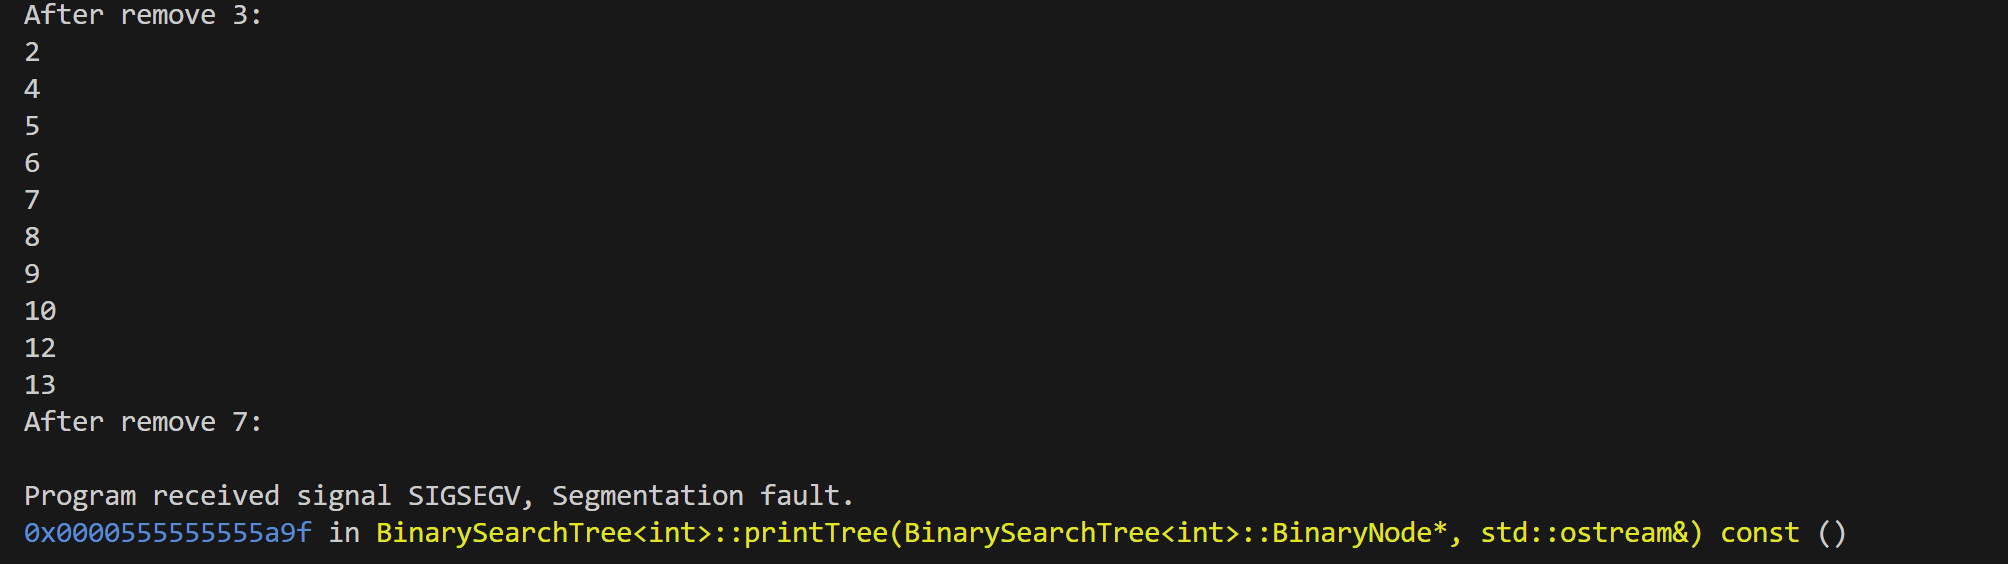
\includegraphics[width=0.8\textwidth]{Segmentation_fault.png}
        \caption{Segmentation fault}
        \label{fig:Segmentation fault}
    \end{figure}
    当root被删除后,再次调用printTree函数时,会出现段错误。
    所以需要及时对root进行更新。\\
    另外,对于后四种情况,都需要知道将被删除的节点,是其父节点的左子树还是右子树,
    所以需要调用寻亲函数,找到父节点,利用toRemove的节点值与其父节点值进行比较,
    再依据各种情况进行相应的赋nullptr或者指针替换操作,如下所示。\\
    \begin{lstlisting}[language=C++]
        if(x < parent->element)
        parent->left = ...
    else
        parent->right = ...
    \end{lstlisting}

\section{测试函数}
省略插入函数建立树的部分,得到的树应为
\begin{figure}[H]
    \centering
    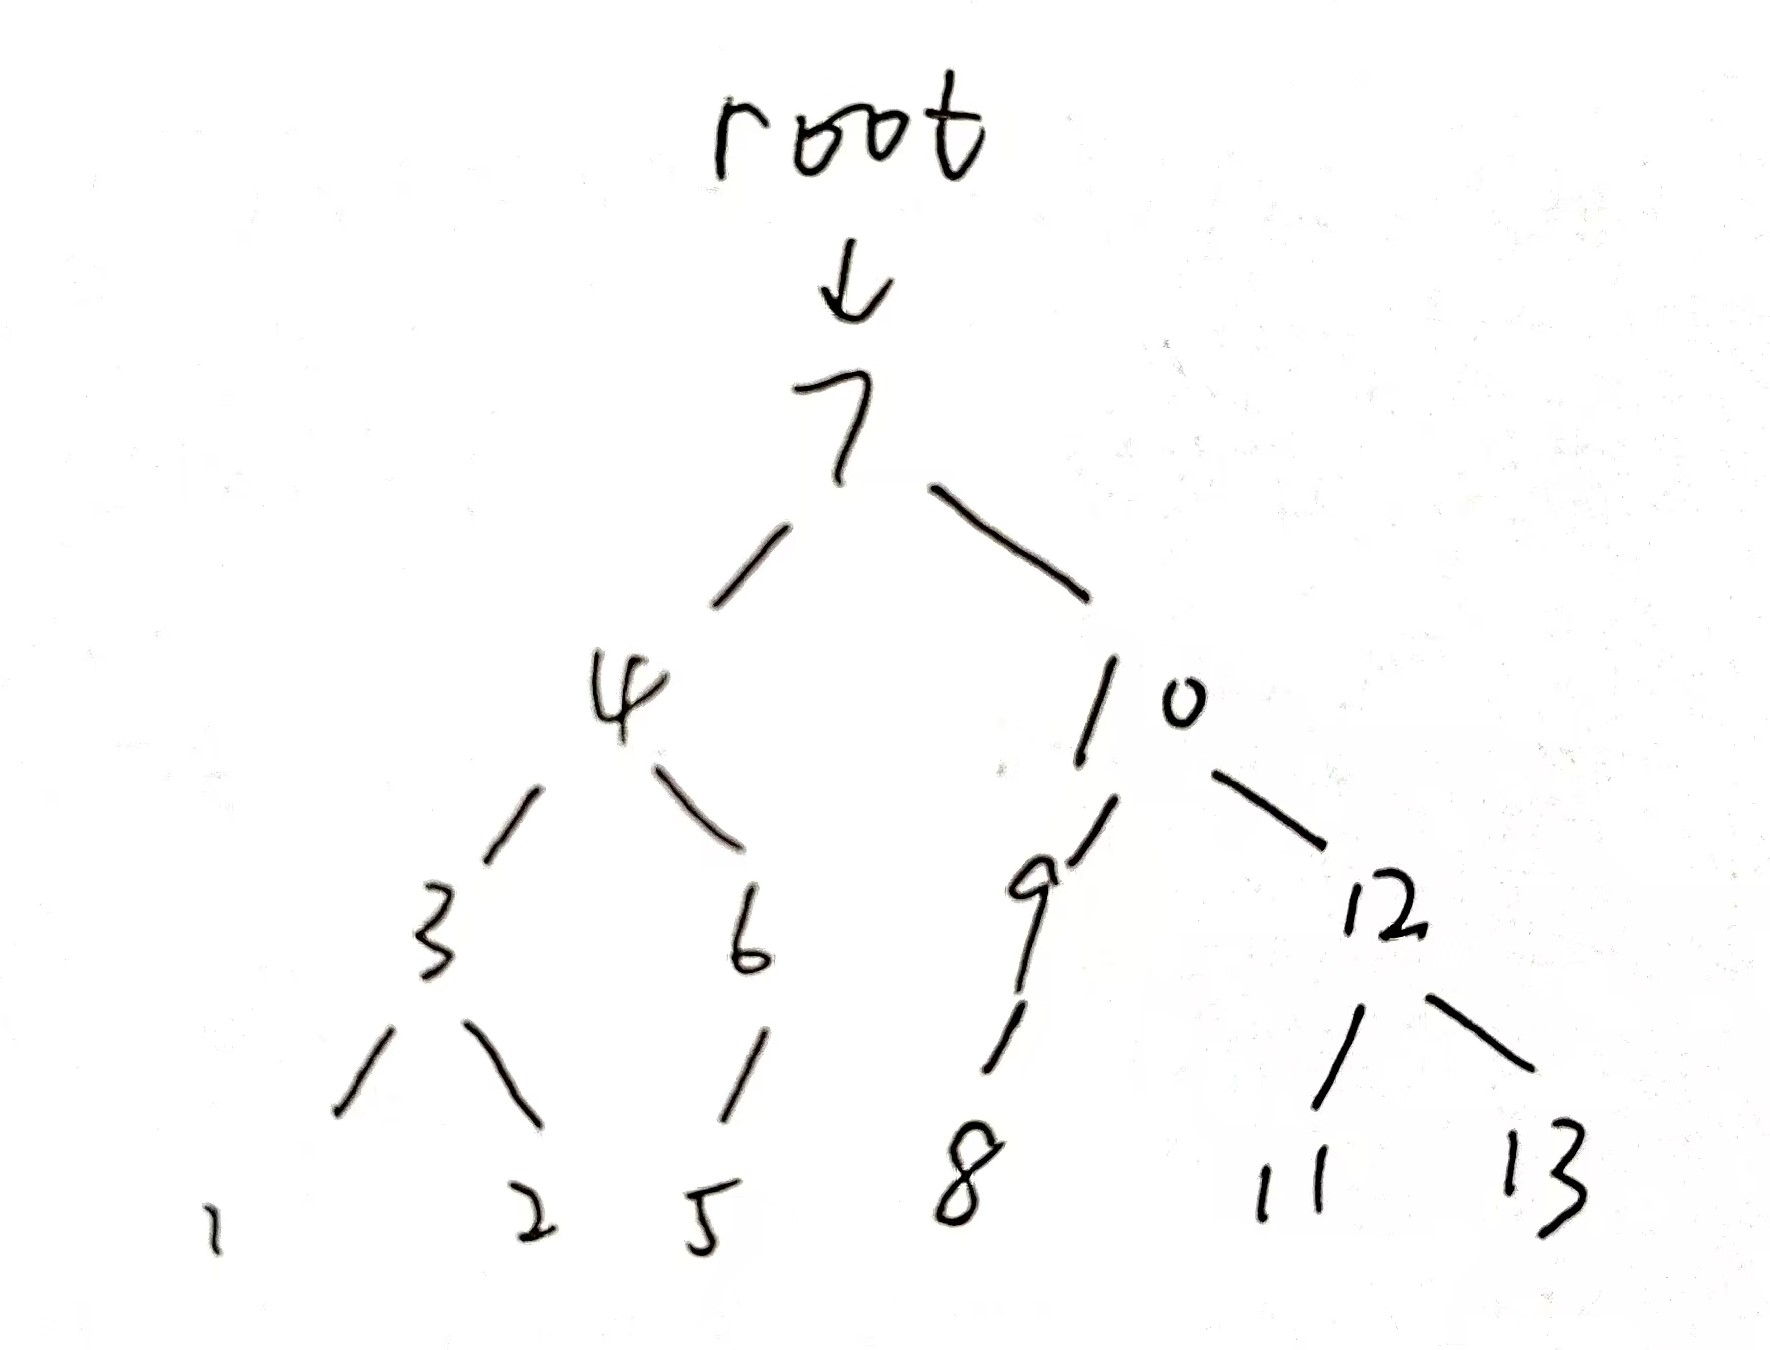
\includegraphics[width=0.4\textwidth]{tree.jpg}
    \caption{BinarySearchTree}
    \label{fig:BinarySearchTree}
\end{figure}
只展示了删除部分的测试函数。完整详见main.cpp文件。
\begin{lstlisting}[language=C++]
    int main()
    {
    BinarySearchTree<int> t;

    t.insert...

    std::cout<<"The tree is:"<<endl;
    t.printTree();

    t.remove(1);//删除叶子节点
    std::cout<<"After remove 1:"<<endl;
    t.printTree();

    t.remove(3);//只有右子节点
    std::cout<<"After remove 3:"<<endl;
    t.printTree();

    t.remove(7);//删除根节点
    std::cout<<"After remove 7:"<<endl;
    t.printTree();

    t.makeEmpty();
    std::cout<<"After makeEmpty:"<<endl;
    t.printTree();
    t.insert...

    std::cout<<"The tree is:"<<endl;
    t.printTree();
    t.remove(9);//只有左子节点
    std::cout<<"After remove 9:"<<endl;
    t.printTree();

    t.remove(10);//有两个子节点
    std::cout<<"After remove 10:"<<endl;
    t.printTree();

    t.remove(3);//有两个子节点,且右子树的最小节点恰为叶子
    std::cout<<"After remove 3:"<<endl;
    t.printTree();
    
    t.insert...

    std::cout<<"The tree is:"<<endl;
    t.printTree();

    t.remove(15);//移除不存在节点
    std::cout<<"After remove 15:"<<endl;
    t.printTree();
    }
\end{lstlisting}
    即分别对上述六种情况逐一进行测试,查看是否会出现错误。
    其中对于有两个节点的情况,还要考虑右子树的最小节点恰为叶子,验证这种情况下detachMin函数能否正常工作。

\section{测试结果}
\begin{verbatim}
summer_hare@localhost:/mnt/d/浙大本科学习/大二上/数据结构与算法分析/My Project/BST$ ./test
The tree is:
1
2
3
4
5
6
7
8
9
10
11
12
13
After remove 1:
2
3
4
5
6
7
8
9
10
11
12
13
After remove 3:
2
4
5
6
7
8
9
10
11
12
13
After remove 7:
2
4
5
6
8
9
10
11
12
13
After makeEmpty:
Empty tree
The tree is:
1
2
3
4
5
6
7
8
9
10
11
12
13
After remove 9:
1
2
3
4
5
6
7
8
10
11
12
13
After remove 10:
1
2
3
4
5
6
7
8
11
12
13
After remove 3:
1
2
4
5
6
7
8
11
12
13
The tree is:
1
2
3
4
5
6
7
8
9
10
11
12
13
After remove 15:
1
2
3
4
5
6
7
8
9
10
11
12
13
\end{verbatim}
    从测试结果来看,删除操作正常,符合理论预期。\\

    使用valgrind检查内存泄漏,结果如下:
\begin{verbatim}
==41042== HEAP SUMMARY:
==41042==     in use at exit: 0 bytes in 0 blocks
==41042==   total heap usage: 227 allocs, 227 frees, 21,159 bytes allocated
==41042== 
==41042== All heap blocks were freed -- no leaks are possible
==41042== 
==41042== For lists of detected and suppressed errors, rerun with: -s
==41042== ERROR SUMMARY: 0 errors from 0 contexts (suppressed: 0 from 0)
\end{verbatim}
    无内存泄漏。
\end{document}